\documentclass[1p]{elsarticle_modified}
%\bibliographystyle{elsarticle-num}

%\usepackage[colorlinks]{hyperref}
%\usepackage{abbrmath_seonhwa} %\Abb, \Ascr, \Acal ,\Abf, \Afrak
\usepackage{amsfonts}
\usepackage{amssymb}
\usepackage{amsmath}
\usepackage{amsthm}
\usepackage{scalefnt}
\usepackage{amsbsy}
\usepackage{kotex}
\usepackage{caption}
\usepackage{subfig}
\usepackage{color}
\usepackage{graphicx}
\usepackage{xcolor} %% white, black, red, green, blue, cyan, magenta, yellow
\usepackage{float}
\usepackage{setspace}
\usepackage{hyperref}

\usepackage{tikz}
\usetikzlibrary{arrows}

\usepackage{multirow}
\usepackage{array} % fixed length table
\usepackage{hhline}

%%%%%%%%%%%%%%%%%%%%%
\makeatletter
\renewcommand*\env@matrix[1][\arraystretch]{%
	\edef\arraystretch{#1}%
	\hskip -\arraycolsep
	\let\@ifnextchar\new@ifnextchar
	\array{*\c@MaxMatrixCols c}}
\makeatother %https://tex.stackexchange.com/questions/14071/how-can-i-increase-the-line-spacing-in-a-matrix
%%%%%%%%%%%%%%%

\usepackage[normalem]{ulem}

\newcommand{\msout}[1]{\ifmmode\text{\sout{\ensuremath{#1}}}\else\sout{#1}\fi}
%SOURCE: \msout is \stkout macro in https://tex.stackexchange.com/questions/20609/strikeout-in-math-mode

\newcommand{\cancel}[1]{
	\ifmmode
	{\color{red}\msout{#1}}
	\else
	{\color{red}\sout{#1}}
	\fi
}

\newcommand{\add}[1]{
	{\color{blue}\uwave{#1}}
}

\newcommand{\replace}[2]{
	\ifmmode
	{\color{red}\msout{#1}}{\color{blue}\uwave{#2}}
	\else
	{\color{red}\sout{#1}}{\color{blue}\uwave{#2}}
	\fi
}

\newcommand{\Sol}{\mathcal{S}} %segment
\newcommand{\D}{D} %diagram
\newcommand{\A}{\mathcal{A}} %arc


%%%%%%%%%%%%%%%%%%%%%%%%%%%%%5 test

\def\sl{\operatorname{\textup{SL}}(2,\Cbb)}
\def\psl{\operatorname{\textup{PSL}}(2,\Cbb)}
\def\quan{\mkern 1mu \triangleright \mkern 1mu}

\theoremstyle{definition}
\newtheorem{thm}{Theorem}[section]
\newtheorem{prop}[thm]{Proposition}
\newtheorem{lem}[thm]{Lemma}
\newtheorem{ques}[thm]{Question}
\newtheorem{cor}[thm]{Corollary}
\newtheorem{defn}[thm]{Definition}
\newtheorem{exam}[thm]{Example}
\newtheorem{rmk}[thm]{Remark}
\newtheorem{alg}[thm]{Algorithm}

\newcommand{\I}{\sqrt{-1}}
\begin{document}

%\begin{frontmatter}
%
%\title{Boundary parabolic representations of knots up to 8 crossings}
%
%%% Group authors per affiliation:
%\author{Yunhi Cho} 
%\address{Department of Mathematics, University of Seoul, Seoul, Korea}
%\ead{yhcho@uos.ac.kr}
%
%
%\author{Seonhwa Kim} %\fnref{s_kim}}
%\address{Center for Geometry and Physics, Institute for Basic Science, Pohang, 37673, Korea}
%\ead{ryeona17@ibs.re.kr}
%
%\author{Hyuk Kim}
%\address{Department of Mathematical Sciences, Seoul National University, Seoul 08826, Korea}
%\ead{hyukkim@snu.ac.kr}
%
%\author{Seokbeom Yoon}
%\address{Department of Mathematical Sciences, Seoul National University, Seoul, 08826,  Korea}
%\ead{sbyoon15@snu.ac.kr}
%
%\begin{abstract}
%We find all boundary parabolic representation of knots up to 8 crossings.
%
%\end{abstract}
%\begin{keyword}
%    \MSC[2010] 57M25 
%\end{keyword}
%
%\end{frontmatter}

%\linenumbers
%\tableofcontents
%
\newcommand\colored[1]{\textcolor{white}{\rule[-0.35ex]{0.8em}{1.4ex}}\kern-0.8em\color{red} #1}%
%\newcommand\colored[1]{\textcolor{white}{ #1}\kern-2.17ex	\textcolor{white}{ #1}\kern-1.81ex	\textcolor{white}{ #1}\kern-2.15ex\color{red}#1	}

{\Large $\underline{12n_{0485}~(K12n_{0485})}$}

\setlength{\tabcolsep}{10pt}
\renewcommand{\arraystretch}{1.6}
\vspace{1cm}\begin{tabular}{m{100pt}>{\centering\arraybackslash}m{274pt}}
\multirow{5}{120pt}{
	\centering
	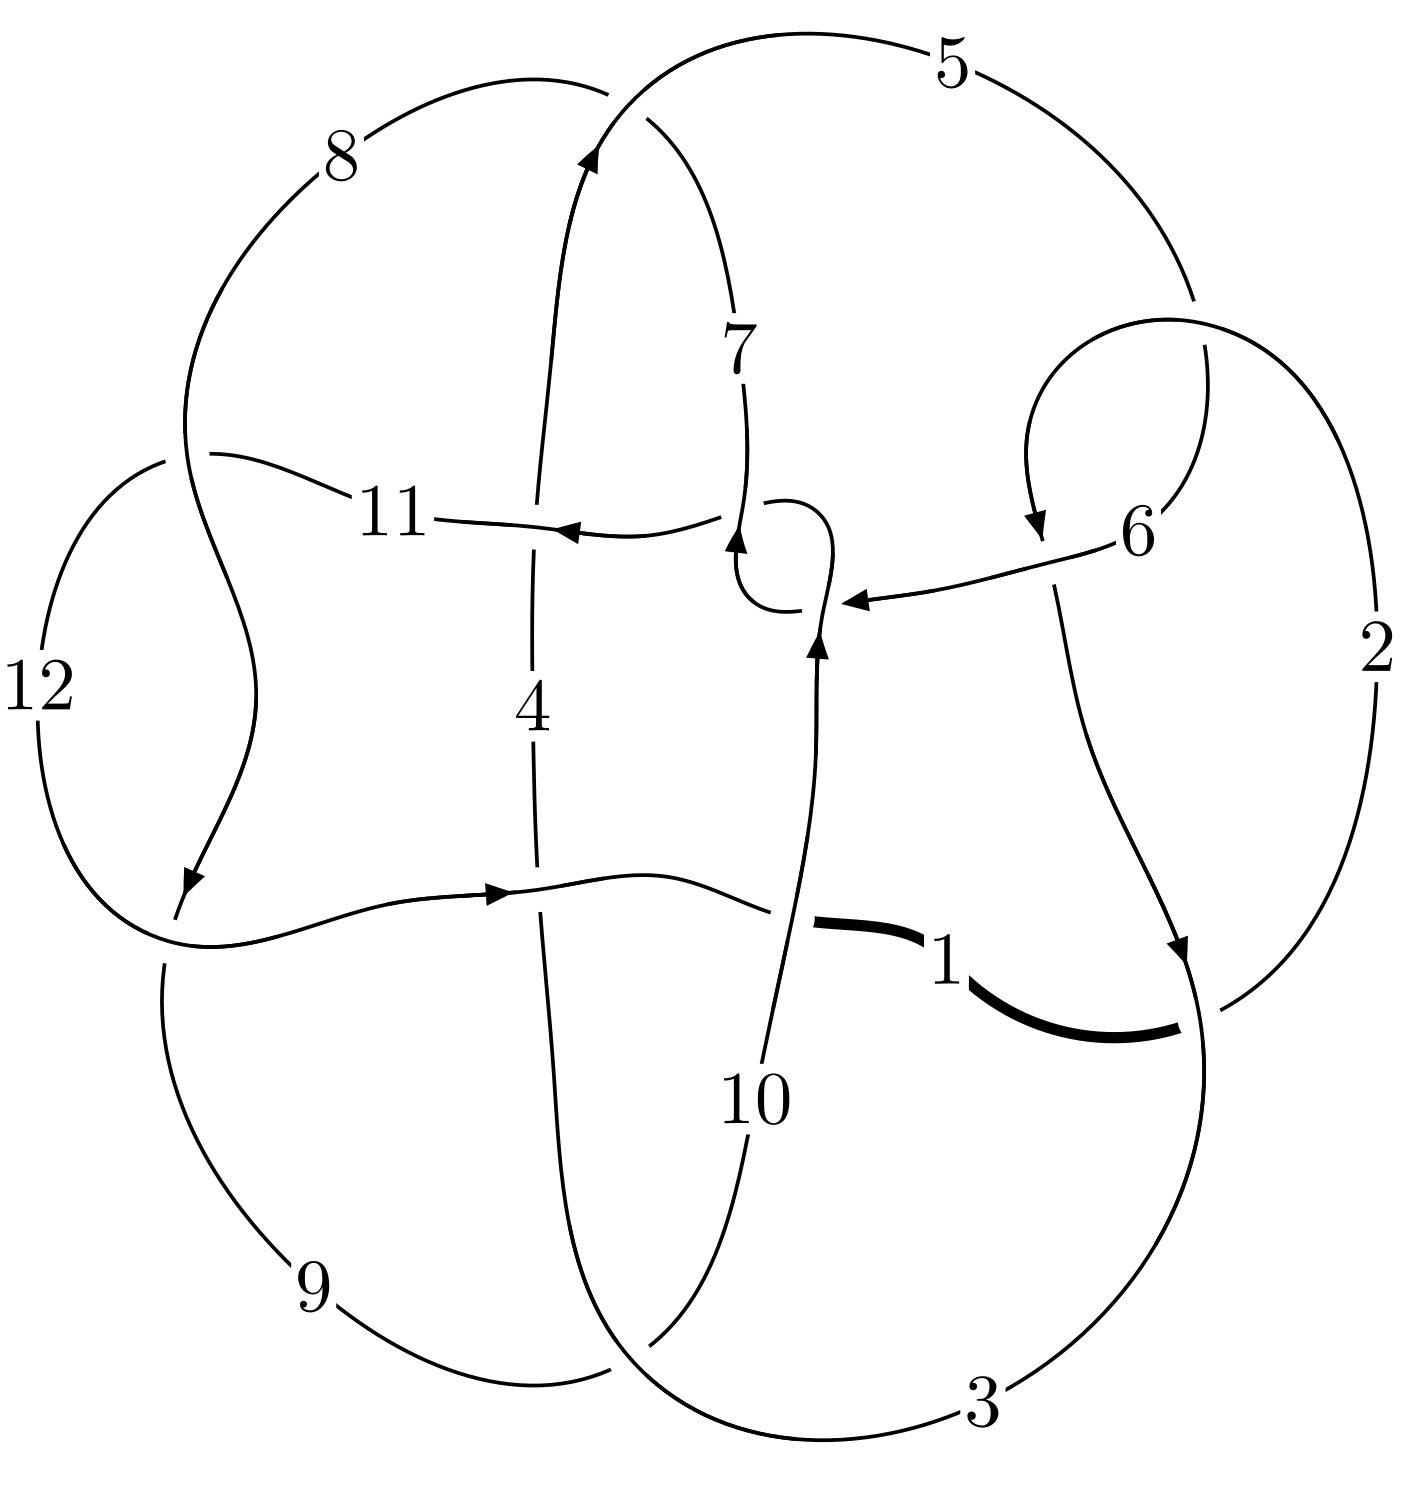
\includegraphics[width=112pt]{../../../GIT/diagram.site/Diagrams/png/2574_12n_0485.png}\\
\ \ \ A knot diagram\footnotemark}&
\allowdisplaybreaks
\textbf{Linearized knot diagam} \\
\cline{2-2}
 &
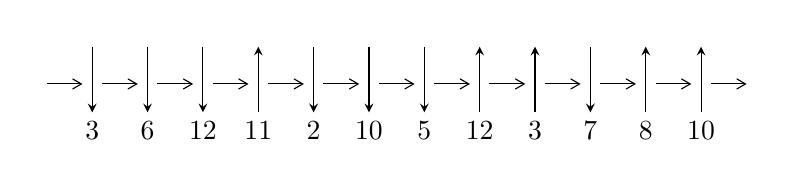
\begin{tikzpicture}[x=20pt, y=17pt]
	% nodes
	\node (C0) at (0, 0) {};
	\node (C1) at (1, 0) {};
	\node (C1U) at (1, +1) {};
	\node (C1D) at (1, -1) {3};

	\node (C2) at (2, 0) {};
	\node (C2U) at (2, +1) {};
	\node (C2D) at (2, -1) {6};

	\node (C3) at (3, 0) {};
	\node (C3U) at (3, +1) {};
	\node (C3D) at (3, -1) {12};

	\node (C4) at (4, 0) {};
	\node (C4U) at (4, +1) {};
	\node (C4D) at (4, -1) {11};

	\node (C5) at (5, 0) {};
	\node (C5U) at (5, +1) {};
	\node (C5D) at (5, -1) {2};

	\node (C6) at (6, 0) {};
	\node (C6U) at (6, +1) {};
	\node (C6D) at (6, -1) {10};

	\node (C7) at (7, 0) {};
	\node (C7U) at (7, +1) {};
	\node (C7D) at (7, -1) {5};

	\node (C8) at (8, 0) {};
	\node (C8U) at (8, +1) {};
	\node (C8D) at (8, -1) {12};

	\node (C9) at (9, 0) {};
	\node (C9U) at (9, +1) {};
	\node (C9D) at (9, -1) {3};

	\node (C10) at (10, 0) {};
	\node (C10U) at (10, +1) {};
	\node (C10D) at (10, -1) {7};

	\node (C11) at (11, 0) {};
	\node (C11U) at (11, +1) {};
	\node (C11D) at (11, -1) {8};

	\node (C12) at (12, 0) {};
	\node (C12U) at (12, +1) {};
	\node (C12D) at (12, -1) {10};
	\node (C13) at (13, 0) {};

	% arrows
	\draw[->,>={angle 60}]
	(C0) edge (C1) (C1) edge (C2) (C2) edge (C3) (C3) edge (C4) (C4) edge (C5) (C5) edge (C6) (C6) edge (C7) (C7) edge (C8) (C8) edge (C9) (C9) edge (C10) (C10) edge (C11) (C11) edge (C12) (C12) edge (C13) ;	\draw[->,>=stealth]
	(C1U) edge (C1D) (C2U) edge (C2D) (C3U) edge (C3D) (C4D) edge (C4U) (C5U) edge (C5D) (C6U) edge (C6D) (C7U) edge (C7D) (C8D) edge (C8U) (C9D) edge (C9U) (C10U) edge (C10D) (C11D) edge (C11U) (C12D) edge (C12U) ;
	\end{tikzpicture} \\
\hhline{~~} \\& 
\textbf{Solving Sequence} \\ \cline{2-2} 
 &
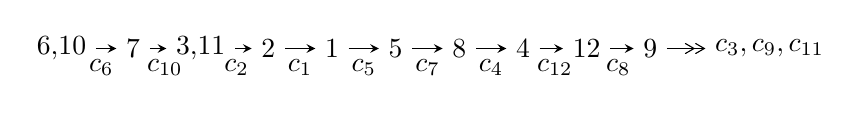
\begin{tikzpicture}[x=23pt, y=7pt]
	% node
	\node (A0) at (-1/8, 0) {6,10};
	\node (A1) at (1, 0) {7};
	\node (A2) at (33/16, 0) {3,11};
	\node (A3) at (25/8, 0) {2};
	\node (A4) at (33/8, 0) {1};
	\node (A5) at (41/8, 0) {5};
	\node (A6) at (49/8, 0) {8};
	\node (A7) at (57/8, 0) {4};
	\node (A8) at (65/8, 0) {12};
	\node (A9) at (73/8, 0) {9};
	\node (C1) at (1/2, -1) {$c_{6}$};
	\node (C2) at (3/2, -1) {$c_{10}$};
	\node (C3) at (21/8, -1) {$c_{2}$};
	\node (C4) at (29/8, -1) {$c_{1}$};
	\node (C5) at (37/8, -1) {$c_{5}$};
	\node (C6) at (45/8, -1) {$c_{7}$};
	\node (C7) at (53/8, -1) {$c_{4}$};
	\node (C8) at (61/8, -1) {$c_{12}$};
	\node (C9) at (69/8, -1) {$c_{8}$};
	\node (A10) at (11, 0) {$c_{3},c_{9},c_{11}$};

	% edge
	\draw[->,>=stealth]	
	(A0) edge (A1) (A1) edge (A2) (A2) edge (A3) (A3) edge (A4) (A4) edge (A5) (A5) edge (A6) (A6) edge (A7) (A7) edge (A8) (A8) edge (A9) ;
	\draw[->>,>={angle 60}]	
	(A9) edge (A10);
\end{tikzpicture} \\ 

\end{tabular} \\

\footnotetext{
The image of knot diagram is generated by the software ``\textbf{Draw programme}" developed by Andrew Bartholomew(\url{http://www.layer8.co.uk/maths/draw/index.htm\#Running-draw}), where we modified some parts for our purpose(\url{https://github.com/CATsTAILs/LinksPainter}).
}\phantom \\ \newline 
\centering \textbf{Ideals for irreducible components\footnotemark of $X_{\text{par}}$} 
 
\begin{align*}
I^u_{1}&=\langle 
1.68088\times10^{114} u^{49}+4.16169\times10^{114} u^{48}+\cdots+7.67515\times10^{115} b+4.28407\times10^{115},\\
\phantom{I^u_{1}}&\phantom{= \langle  }-6.82277\times10^{115} u^{49}-1.30399\times10^{116} u^{48}+\cdots+5.37260\times10^{116} a+7.15218\times10^{117},\\
\phantom{I^u_{1}}&\phantom{= \langle  }u^{50}+2 u^{49}+\cdots-457 u-23\rangle \\
I^u_{2}&=\langle 
-326316 u^{14}-428568 u^{13}+\cdots+738005 b-1963248,\\
\phantom{I^u_{2}}&\phantom{= \langle  }-516082 u^{14}-337061 u^{13}+\cdots+738005 a-2248216,\\
\phantom{I^u_{2}}&\phantom{= \langle  }u^{15}+u^{14}-6 u^{13}-13 u^{12}+11 u^{11}+48 u^{10}+15 u^9-72 u^8-69 u^7+41 u^6+80 u^5+u^4-39 u^3-6 u^2+7 u-1\rangle \\
\\
\end{align*}
\raggedright * 2 irreducible components of $\dim_{\mathbb{C}}=0$, with total 65 representations.\\
\footnotetext{All coefficients of polynomials are rational numbers. But the coefficients are sometimes approximated in decimal forms when there is not enough margin.}
\newpage
\renewcommand{\arraystretch}{1}
\centering \section*{I. $I^u_{1}= \langle 1.68\times10^{114} u^{49}+4.16\times10^{114} u^{48}+\cdots+7.68\times10^{115} b+4.28\times10^{115},\;-6.82\times10^{115} u^{49}-1.30\times10^{116} u^{48}+\cdots+5.37\times10^{116} a+7.15\times10^{117},\;u^{50}+2 u^{49}+\cdots-457 u-23 \rangle$}
\flushleft \textbf{(i) Arc colorings}\\
\begin{tabular}{m{7pt} m{180pt} m{7pt} m{180pt} }
\flushright $a_{6}=$&$\begin{pmatrix}1\\0\end{pmatrix}$ \\
\flushright $a_{10}=$&$\begin{pmatrix}0\\u\end{pmatrix}$ \\
\flushright $a_{7}=$&$\begin{pmatrix}1\\u^2\end{pmatrix}$ \\
\flushright $a_{3}=$&$\begin{pmatrix}0.126992 u^{49}+0.242711 u^{48}+\cdots-212.139 u-13.3123\\-0.0219003 u^{49}-0.0542229 u^{48}+\cdots-4.04389 u-0.558174\end{pmatrix}$ \\
\flushright $a_{11}=$&$\begin{pmatrix}- u\\- u^3+u\end{pmatrix}$ \\
\flushright $a_{2}=$&$\begin{pmatrix}0.105092 u^{49}+0.188488 u^{48}+\cdots-216.183 u-13.8705\\-0.0219003 u^{49}-0.0542229 u^{48}+\cdots-4.04389 u-0.558174\end{pmatrix}$ \\
\flushright $a_{1}=$&$\begin{pmatrix}-0.0244401 u^{49}-0.0544173 u^{48}+\cdots+64.2416 u+6.94455\\0.0202777 u^{49}+0.0488855 u^{48}+\cdots-0.453421 u-0.822925\end{pmatrix}$ \\
\flushright $a_{5}=$&$\begin{pmatrix}0.125355 u^{49}+0.236460 u^{48}+\cdots-229.828 u-15.6829\\0.0231342 u^{49}+0.0609480 u^{48}+\cdots+55.0377 u+2.61238\end{pmatrix}$ \\
\flushright $a_{8}=$&$\begin{pmatrix}-0.121315 u^{49}-0.239466 u^{48}+\cdots+307.315 u+24.6209\\0.0144984 u^{49}+0.0160292 u^{48}+\cdots-43.7020 u-2.79868\end{pmatrix}$ \\
\flushright $a_{4}=$&$\begin{pmatrix}0.111866 u^{49}+0.205756 u^{48}+\cdots-237.020 u-15.8895\\0.0326281 u^{49}+0.0837666 u^{48}+\cdots+60.2174 u+2.73337\end{pmatrix}$ \\
\flushright $a_{12}=$&$\begin{pmatrix}-0.0244401 u^{49}-0.0544173 u^{48}+\cdots+64.2416 u+6.94455\\0.0232371 u^{49}+0.0518221 u^{48}+\cdots-3.54599 u-0.950278\end{pmatrix}$ \\
\flushright $a_{9}=$&$\begin{pmatrix}-0.143868 u^{49}-0.280796 u^{48}+\cdots+334.339 u+27.3191\\0.0289298 u^{49}+0.0544418 u^{48}+\cdots-28.4198 u-2.35108\end{pmatrix}$\\&\end{tabular}
\flushleft \textbf{(ii) Obstruction class $= -1$}\\~\\
\flushleft \textbf{(iii) Cusp Shapes $= -0.270594 u^{49}-0.467859 u^{48}+\cdots-63.7985 u-8.23325$}\\~\\
\newpage\renewcommand{\arraystretch}{1}
\flushleft \textbf{(iv) u-Polynomials at the component}\newline \\
\begin{tabular}{m{50pt}|m{274pt}}
Crossings & \hspace{64pt}u-Polynomials at each crossing \\
\hline $$\begin{aligned}c_{1}\end{aligned}$$&$\begin{aligned}
&u^{50}+38 u^{49}+\cdots-888 u+361
\end{aligned}$\\
\hline $$\begin{aligned}c_{2},c_{5}\end{aligned}$$&$\begin{aligned}
&u^{50}-19 u^{48}+\cdots+86 u+19
\end{aligned}$\\
\hline $$\begin{aligned}c_{3}\end{aligned}$$&$\begin{aligned}
&u^{50}-9 u^{49}+\cdots+7672 u+449
\end{aligned}$\\
\hline $$\begin{aligned}c_{4}\end{aligned}$$&$\begin{aligned}
&u^{50}-3 u^{49}+\cdots-316 u-239
\end{aligned}$\\
\hline $$\begin{aligned}c_{6},c_{10}\end{aligned}$$&$\begin{aligned}
&u^{50}+2 u^{49}+\cdots-457 u-23
\end{aligned}$\\
\hline $$\begin{aligned}c_{7}\end{aligned}$$&$\begin{aligned}
&u^{50}-5 u^{49}+\cdots-18 u+1
\end{aligned}$\\
\hline $$\begin{aligned}c_{8},c_{11}\end{aligned}$$&$\begin{aligned}
&u^{50}-3 u^{49}+\cdots+7 u+1
\end{aligned}$\\
\hline $$\begin{aligned}c_{9}\end{aligned}$$&$\begin{aligned}
&u^{50}- u^{49}+\cdots-48 u-119
\end{aligned}$\\
\hline $$\begin{aligned}c_{12}\end{aligned}$$&$\begin{aligned}
&u^{50}+3 u^{49}+\cdots-36385 u-1997
\end{aligned}$\\
\hline
\end{tabular}\\~\\
\newpage\renewcommand{\arraystretch}{1}
\flushleft \textbf{(v) Riley Polynomials at the component}\newline \\
\begin{tabular}{m{50pt}|m{274pt}}
Crossings & \hspace{64pt}Riley Polynomials at each crossing \\
\hline $$\begin{aligned}c_{1}\end{aligned}$$&$\begin{aligned}
&y^{50}-42 y^{49}+\cdots+7137572 y+130321
\end{aligned}$\\
\hline $$\begin{aligned}c_{2},c_{5}\end{aligned}$$&$\begin{aligned}
&y^{50}-38 y^{49}+\cdots+888 y+361
\end{aligned}$\\
\hline $$\begin{aligned}c_{3}\end{aligned}$$&$\begin{aligned}
&y^{50}-85 y^{49}+\cdots-26826128 y+201601
\end{aligned}$\\
\hline $$\begin{aligned}c_{4}\end{aligned}$$&$\begin{aligned}
&y^{50}+31 y^{49}+\cdots+1567408 y+57121
\end{aligned}$\\
\hline $$\begin{aligned}c_{6},c_{10}\end{aligned}$$&$\begin{aligned}
&y^{50}-50 y^{49}+\cdots-75863 y+529
\end{aligned}$\\
\hline $$\begin{aligned}c_{7}\end{aligned}$$&$\begin{aligned}
&y^{50}+7 y^{49}+\cdots-88 y+1
\end{aligned}$\\
\hline $$\begin{aligned}c_{8},c_{11}\end{aligned}$$&$\begin{aligned}
&y^{50}-9 y^{49}+\cdots-19 y+1
\end{aligned}$\\
\hline $$\begin{aligned}c_{9}\end{aligned}$$&$\begin{aligned}
&y^{50}+57 y^{49}+\cdots+139782 y+14161
\end{aligned}$\\
\hline $$\begin{aligned}c_{12}\end{aligned}$$&$\begin{aligned}
&y^{50}+95 y^{49}+\cdots-251387363 y+3988009
\end{aligned}$\\
\hline
\end{tabular}\\~\\
\newpage\flushleft \textbf{(vi) Complex Volumes and Cusp Shapes}
$$\begin{array}{c|c|c}  
\text{Solutions to }I^u_{1}& \I (\text{vol} + \sqrt{-1}CS) & \text{Cusp shape}\\
 \hline 
\begin{aligned}
u &= \phantom{-}0.962392\phantom{ +0.000000I} \\
a &= -1.01045\phantom{ +0.000000I} \\
b &= -1.32074\phantom{ +0.000000I}\end{aligned}
 & -2.96141\phantom{ +0.000000I} & \phantom{-}2.27250\phantom{ +0.000000I} \\ \hline\begin{aligned}
u &= -0.914795 + 0.294994 I \\
a &= \phantom{-}0.348985 - 1.244120 I \\
b &= -0.336309 + 0.574877 I\end{aligned}
 & -1.75231 + 1.61093 I & -2.00000 - 4.17914 I \\ \hline\begin{aligned}
u &= -0.914795 - 0.294994 I \\
a &= \phantom{-}0.348985 + 1.244120 I \\
b &= -0.336309 - 0.574877 I\end{aligned}
 & -1.75231 - 1.61093 I & -2.00000 + 4.17914 I \\ \hline\begin{aligned}
u &= \phantom{-}0.188071 + 0.934572 I \\
a &= -1.32544 - 0.55559 I \\
b &= -0.330034 + 0.374073 I\end{aligned}
 & -3.45737 - 4.06670 I & \phantom{-}                -6
0.298116 + 0. 10   I\phantom{ +0.000000I} \\ \hline\begin{aligned}
u &= \phantom{-}0.188071 - 0.934572 I \\
a &= -1.32544 + 0.55559 I \\
b &= -0.330034 - 0.374073 I\end{aligned}
 & -3.45737 + 4.06670 I & \phantom{-}                -6
0.298116 + 0. 10   I\phantom{ +0.000000I} \\ \hline\begin{aligned}
u &= -1.063020 + 0.238205 I \\
a &= \phantom{-}0.513483 - 0.668053 I \\
b &= -0.219406 + 0.431806 I\end{aligned}
 & -1.88900 + 1.18238 I & \phantom{-0.000000 } 0 \\ \hline\begin{aligned}
u &= -1.063020 - 0.238205 I \\
a &= \phantom{-}0.513483 + 0.668053 I \\
b &= -0.219406 - 0.431806 I\end{aligned}
 & -1.88900 - 1.18238 I & \phantom{-0.000000 } 0 \\ \hline\begin{aligned}
u &= -1.12876\phantom{ +0.000000I} \\
a &= -2.19559\phantom{ +0.000000I} \\
b &= -1.15007\phantom{ +0.000000I}\end{aligned}
 & -3.84446\phantom{ +0.000000I} & \phantom{-}56.7750\phantom{ +0.000000I} \\ \hline\begin{aligned}
u &= -0.201542 + 1.118180 I \\
a &= -0.163469 + 0.515966 I \\
b &= \phantom{-}0.939070 - 0.303988 I\end{aligned}
 & -0.56528 + 3.67939 I & \phantom{-0.000000 } 0. - 8.30272 I \\ \hline\begin{aligned}
u &= -0.201542 - 1.118180 I \\
a &= -0.163469 - 0.515966 I \\
b &= \phantom{-}0.939070 + 0.303988 I\end{aligned}
 & -0.56528 - 3.67939 I & \phantom{-0.000000 -}0. + 8.30272 I\\
 \hline 
 \end{array}$$\newpage$$\begin{array}{c|c|c}  
\text{Solutions to }I^u_{1}& \I (\text{vol} + \sqrt{-1}CS) & \text{Cusp shape}\\
 \hline 
\begin{aligned}
u &= -1.133680 + 0.426918 I \\
a &= \phantom{-}0.19890 - 1.42670 I \\
b &= -1.125150 + 0.186429 I\end{aligned}
 & -3.75163 + 1.13848 I & \phantom{-0.000000 } 0 \\ \hline\begin{aligned}
u &= -1.133680 - 0.426918 I \\
a &= \phantom{-}0.19890 + 1.42670 I \\
b &= -1.125150 - 0.186429 I\end{aligned}
 & -3.75163 - 1.13848 I & \phantom{-0.000000 } 0 \\ \hline\begin{aligned}
u &= \phantom{-}1.166960 + 0.482292 I \\
a &= -0.242984 + 0.621460 I \\
b &= \phantom{-}0.025892 - 0.730255 I\end{aligned}
 & -1.46117 - 5.17618 I & \phantom{-0.000000 } 0 \\ \hline\begin{aligned}
u &= \phantom{-}1.166960 - 0.482292 I \\
a &= -0.242984 - 0.621460 I \\
b &= \phantom{-}0.025892 + 0.730255 I\end{aligned}
 & -1.46117 + 5.17618 I & \phantom{-0.000000 } 0 \\ \hline\begin{aligned}
u &= \phantom{-}1.161870 + 0.501646 I \\
a &= \phantom{-}0.174398 - 0.201602 I \\
b &= \phantom{-}0.852089 - 0.342703 I\end{aligned}
 & \phantom{-}2.18914 + 1.57391 I & \phantom{-0.000000 } 0 \\ \hline\begin{aligned}
u &= \phantom{-}1.161870 - 0.501646 I \\
a &= \phantom{-}0.174398 + 0.201602 I \\
b &= \phantom{-}0.852089 + 0.342703 I\end{aligned}
 & \phantom{-}2.18914 - 1.57391 I & \phantom{-0.000000 } 0 \\ \hline\begin{aligned}
u &= \phantom{-}0.279120 + 0.649040 I \\
a &= \phantom{-}0.526491 - 0.708843 I \\
b &= \phantom{-}0.200176 + 0.379822 I\end{aligned}
 & \phantom{-}1.27220 + 0.82528 I & \phantom{-}4.71608 - 1.63337 I \\ \hline\begin{aligned}
u &= \phantom{-}0.279120 - 0.649040 I \\
a &= \phantom{-}0.526491 + 0.708843 I \\
b &= \phantom{-}0.200176 - 0.379822 I\end{aligned}
 & \phantom{-}1.27220 - 0.82528 I & \phantom{-}4.71608 + 1.63337 I \\ \hline\begin{aligned}
u &= -1.406050 + 0.128958 I \\
a &= -0.090166 + 1.145330 I \\
b &= \phantom{-}1.49695 - 0.61870 I\end{aligned}
 & -13.59260 - 1.25874 I & \phantom{-0.000000 } 0 \\ \hline\begin{aligned}
u &= -1.406050 - 0.128958 I \\
a &= -0.090166 - 1.145330 I \\
b &= \phantom{-}1.49695 + 0.61870 I\end{aligned}
 & -13.59260 + 1.25874 I & \phantom{-0.000000 } 0\\
 \hline 
 \end{array}$$\newpage$$\begin{array}{c|c|c}  
\text{Solutions to }I^u_{1}& \I (\text{vol} + \sqrt{-1}CS) & \text{Cusp shape}\\
 \hline 
\begin{aligned}
u &= -1.40806 + 0.28799 I \\
a &= -0.208667 + 0.877622 I \\
b &= -0.799188 - 0.695079 I\end{aligned}
 & -1.71585 - 2.64303 I & \phantom{-0.000000 } 0 \\ \hline\begin{aligned}
u &= -1.40806 - 0.28799 I \\
a &= -0.208667 - 0.877622 I \\
b &= -0.799188 + 0.695079 I\end{aligned}
 & -1.71585 + 2.64303 I & \phantom{-0.000000 } 0 \\ \hline\begin{aligned}
u &= \phantom{-}1.38930 + 0.44579 I \\
a &= \phantom{-}0.530144 - 0.813142 I \\
b &= \phantom{-}1.290420 + 0.327880 I\end{aligned}
 & -5.44067 - 9.04729 I & \phantom{-0.000000 } 0 \\ \hline\begin{aligned}
u &= \phantom{-}1.38930 - 0.44579 I \\
a &= \phantom{-}0.530144 + 0.813142 I \\
b &= \phantom{-}1.290420 - 0.327880 I\end{aligned}
 & -5.44067 + 9.04729 I & \phantom{-0.000000 } 0 \\ \hline\begin{aligned}
u &= \phantom{-}0.499788 + 0.001448 I \\
a &= -0.058887 - 0.899672 I \\
b &= \phantom{-}0.908853 + 0.846009 I\end{aligned}
 & \phantom{-}4.40130 - 3.14257 I & -9.86497 + 6.30227 I \\ \hline\begin{aligned}
u &= \phantom{-}0.499788 - 0.001448 I \\
a &= -0.058887 + 0.899672 I \\
b &= \phantom{-}0.908853 - 0.846009 I\end{aligned}
 & \phantom{-}4.40130 + 3.14257 I & -9.86497 - 6.30227 I \\ \hline\begin{aligned}
u &= -1.47559 + 0.28198 I \\
a &= -0.081256 + 1.075060 I \\
b &= \phantom{-}0.042685 - 1.259730 I\end{aligned}
 & -9.03640 + 8.03955 I & \phantom{-0.000000 } 0 \\ \hline\begin{aligned}
u &= -1.47559 - 0.28198 I \\
a &= -0.081256 - 1.075060 I \\
b &= \phantom{-}0.042685 + 1.259730 I\end{aligned}
 & -9.03640 - 8.03955 I & \phantom{-0.000000 } 0 \\ \hline\begin{aligned}
u &= -0.187501 + 0.455490 I \\
a &= -3.04218 + 1.68708 I \\
b &= \phantom{-}1.382520 + 0.000995 I\end{aligned}
 & -9.25542 + 3.21801 I & -8.68028 - 2.26278 I \\ \hline\begin{aligned}
u &= -0.187501 - 0.455490 I \\
a &= -3.04218 - 1.68708 I \\
b &= \phantom{-}1.382520 - 0.000995 I\end{aligned}
 & -9.25542 - 3.21801 I & -8.68028 + 2.26278 I\\
 \hline 
 \end{array}$$\newpage$$\begin{array}{c|c|c}  
\text{Solutions to }I^u_{1}& \I (\text{vol} + \sqrt{-1}CS) & \text{Cusp shape}\\
 \hline 
\begin{aligned}
u &= \phantom{-}1.50019 + 0.27239 I \\
a &= -0.051146 - 1.185010 I \\
b &= \phantom{-}1.44274 + 0.53398 I\end{aligned}
 & -15.1134 - 6.2855 I & \phantom{-0.000000 } 0 \\ \hline\begin{aligned}
u &= \phantom{-}1.50019 - 0.27239 I \\
a &= -0.051146 + 1.185010 I \\
b &= \phantom{-}1.44274 - 0.53398 I\end{aligned}
 & -15.1134 + 6.2855 I & \phantom{-0.000000 } 0 \\ \hline\begin{aligned}
u &= \phantom{-}1.53985 + 0.12206 I \\
a &= -0.124852 - 1.057310 I \\
b &= -0.048220 + 1.175680 I\end{aligned}
 & -10.37170 + 0.19283 I & \phantom{-0.000000 } 0 \\ \hline\begin{aligned}
u &= \phantom{-}1.53985 - 0.12206 I \\
a &= -0.124852 + 1.057310 I \\
b &= -0.048220 - 1.175680 I\end{aligned}
 & -10.37170 - 0.19283 I & \phantom{-0.000000 } 0 \\ \hline\begin{aligned}
u &= \phantom{-}1.54597 + 0.25810 I \\
a &= -0.163723 - 0.343395 I \\
b &= -1.314650 + 0.219888 I\end{aligned}
 & -5.75356 - 1.82353 I & \phantom{-0.000000 } 0 \\ \hline\begin{aligned}
u &= \phantom{-}1.54597 - 0.25810 I \\
a &= -0.163723 + 0.343395 I \\
b &= -1.314650 - 0.219888 I\end{aligned}
 & -5.75356 + 1.82353 I & \phantom{-0.000000 } 0 \\ \hline\begin{aligned}
u &= -1.37962 + 0.95465 I \\
a &= -0.320379 + 0.766815 I \\
b &= \phantom{-}1.42544 - 0.21562 I\end{aligned}
 & -7.41648 + 4.49387 I & \phantom{-0.000000 } 0 \\ \hline\begin{aligned}
u &= -1.37962 - 0.95465 I \\
a &= -0.320379 - 0.766815 I \\
b &= \phantom{-}1.42544 + 0.21562 I\end{aligned}
 & -7.41648 - 4.49387 I & \phantom{-0.000000 } 0 \\ \hline\begin{aligned}
u &= -0.176458 + 0.261015 I \\
a &= \phantom{-}2.19741 - 2.19418 I \\
b &= -0.984299 - 0.645971 I\end{aligned}
 & \phantom{-}2.84989 - 2.54700 I & \phantom{-}0.20027 + 2.87410 I \\ \hline\begin{aligned}
u &= -0.176458 - 0.261015 I \\
a &= \phantom{-}2.19741 + 2.19418 I \\
b &= -0.984299 + 0.645971 I\end{aligned}
 & \phantom{-}2.84989 + 2.54700 I & \phantom{-}0.20027 - 2.87410 I\\
 \hline 
 \end{array}$$\newpage$$\begin{array}{c|c|c}  
\text{Solutions to }I^u_{1}& \I (\text{vol} + \sqrt{-1}CS) & \text{Cusp shape}\\
 \hline 
\begin{aligned}
u &= -1.67091 + 0.40185 I \\
a &= \phantom{-}0.133031 + 0.469663 I \\
b &= \phantom{-}1.308980 - 0.234411 I\end{aligned}
 & -6.47062 + 3.76881 I & \phantom{-0.000000 } 0 \\ \hline\begin{aligned}
u &= -1.67091 - 0.40185 I \\
a &= \phantom{-}0.133031 - 0.469663 I \\
b &= \phantom{-}1.308980 + 0.234411 I\end{aligned}
 & -6.47062 - 3.76881 I & \phantom{-0.000000 } 0 \\ \hline\begin{aligned}
u &= -1.73086 + 0.55706 I \\
a &= \phantom{-}0.105414 - 0.948189 I \\
b &= -1.46194 + 0.56733 I\end{aligned}
 & -13.8255 + 14.4892 I & \phantom{-0.000000 } 0 \\ \hline\begin{aligned}
u &= -1.73086 - 0.55706 I \\
a &= \phantom{-}0.105414 + 0.948189 I \\
b &= -1.46194 - 0.56733 I\end{aligned}
 & -13.8255 - 14.4892 I & \phantom{-0.000000 } 0 \\ \hline\begin{aligned}
u &= \phantom{-}1.81370 + 0.37242 I \\
a &= \phantom{-}0.097510 + 0.883592 I \\
b &= -1.40613 - 0.59107 I\end{aligned}
 & -14.6308 - 6.0935 I & \phantom{-0.000000 } 0 \\ \hline\begin{aligned}
u &= \phantom{-}1.81370 - 0.37242 I \\
a &= \phantom{-}0.097510 - 0.883592 I \\
b &= -1.40613 + 0.59107 I\end{aligned}
 & -14.6308 + 6.0935 I & \phantom{-0.000000 } 0 \\ \hline\begin{aligned}
u &= -0.1120250 + 0.0235911 I \\
a &= \phantom{-}5.77586 - 3.15149 I \\
b &= -0.849378 + 0.151074 I\end{aligned}
 & -1.45480 + 0.34218 I & -6.89829 + 0.51719 I \\ \hline\begin{aligned}
u &= -0.1120250 - 0.0235911 I \\
a &= \phantom{-}5.77586 + 3.15149 I \\
b &= -0.849378 - 0.151074 I\end{aligned}
 & -1.45480 - 0.34218 I & -6.89829 - 0.51719 I \\ \hline\begin{aligned}
u &= \phantom{-}0.85847 + 1.91212 I \\
a &= \phantom{-}0.591928 + 0.361934 I \\
b &= -1.205700 - 0.185859 I\end{aligned}
 & -6.19255 - 6.25623 I & \phantom{-0.000000 } 0 \\ \hline\begin{aligned}
u &= \phantom{-}0.85847 - 1.91212 I \\
a &= \phantom{-}0.591928 - 0.361934 I \\
b &= -1.205700 + 0.185859 I\end{aligned}
 & -6.19255 + 6.25623 I & \phantom{-0.000000 } 0\\
 \hline 
 \end{array}$$\newpage\newpage\renewcommand{\arraystretch}{1}
\centering \section*{II. $I^u_{2}= \langle -3.26\times10^{5} u^{14}-4.29\times10^{5} u^{13}+\cdots+7.38\times10^{5} b-1.96\times10^{6},\;-5.16\times10^{5} u^{14}-3.37\times10^{5} u^{13}+\cdots+7.38\times10^{5} a-2.25\times10^{6},\;u^{15}+u^{14}+\cdots+7 u-1 \rangle$}
\flushleft \textbf{(i) Arc colorings}\\
\begin{tabular}{m{7pt} m{180pt} m{7pt} m{180pt} }
\flushright $a_{6}=$&$\begin{pmatrix}1\\0\end{pmatrix}$ \\
\flushright $a_{10}=$&$\begin{pmatrix}0\\u\end{pmatrix}$ \\
\flushright $a_{7}=$&$\begin{pmatrix}1\\u^2\end{pmatrix}$ \\
\flushright $a_{3}=$&$\begin{pmatrix}0.699293 u^{14}+0.456719 u^{13}+\cdots-8.14388 u+3.04634\\0.442160 u^{14}+0.580712 u^{13}+\cdots-4.70877 u+2.66021\end{pmatrix}$ \\
\flushright $a_{11}=$&$\begin{pmatrix}- u\\- u^3+u\end{pmatrix}$ \\
\flushright $a_{2}=$&$\begin{pmatrix}1.14145 u^{14}+1.03743 u^{13}+\cdots-12.8527 u+5.70655\\0.442160 u^{14}+0.580712 u^{13}+\cdots-4.70877 u+2.66021\end{pmatrix}$ \\
\flushright $a_{1}=$&$\begin{pmatrix}0.701112 u^{14}+0.979793 u^{13}+\cdots-10.1395 u+6.46055\\-0.0843436 u^{14}-0.544892 u^{13}+\cdots+10.4553 u-0.463978\end{pmatrix}$ \\
\flushright $a_{5}=$&$\begin{pmatrix}-1.76423 u^{14}-2.44279 u^{13}+\cdots+26.2734 u-5.77124\\-1.06494 u^{14}-0.986071 u^{13}+\cdots+11.1296 u-3.72490\end{pmatrix}$ \\
\flushright $a_{8}=$&$\begin{pmatrix}-0.840260 u^{14}-0.979408 u^{13}+\cdots+8.72051 u-6.30081\\0.440341 u^{14}+0.0576378 u^{13}+\cdots-2.71316 u-0.753996\end{pmatrix}$ \\
\flushright $a_{4}=$&$\begin{pmatrix}-1.45570 u^{14}-2.40598 u^{13}+\cdots+25.6851 u-5.33526\\-0.956101 u^{14}-1.06517 u^{13}+\cdots+13.9285 u-4.43261\end{pmatrix}$ \\
\flushright $a_{12}=$&$\begin{pmatrix}0.701112 u^{14}+0.979793 u^{13}+\cdots-10.1395 u+6.46055\\-0.446840 u^{14}-0.697475 u^{13}+\cdots+9.20568 u-0.185297\end{pmatrix}$ \\
\flushright $a_{9}=$&$\begin{pmatrix}0.159740 u^{14}+0.0205920 u^{13}+\cdots+2.72051 u-0.300808\\-0.757426 u^{14}-0.700316 u^{13}+\cdots+2.84871 u-0.699293\end{pmatrix}$\\&\end{tabular}
\flushleft \textbf{(ii) Obstruction class $= 1$}\\~\\
\flushleft \textbf{(iii) Cusp Shapes $= -\frac{337434}{738005} u^{14}-\frac{617487}{738005} u^{13}+\cdots+\frac{14750433}{738005} u+\frac{4380108}{738005}$}\\~\\
\newpage\renewcommand{\arraystretch}{1}
\flushleft \textbf{(iv) u-Polynomials at the component}\newline \\
\begin{tabular}{m{50pt}|m{274pt}}
Crossings & \hspace{64pt}u-Polynomials at each crossing \\
\hline $$\begin{aligned}c_{1}\end{aligned}$$&$\begin{aligned}
&u^{15}-9 u^{14}+\cdots+14 u-1
\end{aligned}$\\
\hline $$\begin{aligned}c_{2}\end{aligned}$$&$\begin{aligned}
&u^{15}+u^{14}+\cdots-2 u-1
\end{aligned}$\\
\hline $$\begin{aligned}c_{3}\end{aligned}$$&$\begin{aligned}
&u^{15}+4 u^{14}+\cdots+14 u+1
\end{aligned}$\\
\hline $$\begin{aligned}c_{4}\end{aligned}$$&$\begin{aligned}
&u^{15}+6 u^{13}+\cdots+2 u+1
\end{aligned}$\\
\hline $$\begin{aligned}c_{5}\end{aligned}$$&$\begin{aligned}
&u^{15}- u^{14}+\cdots-2 u+1
\end{aligned}$\\
\hline $$\begin{aligned}c_{6}\end{aligned}$$&$\begin{aligned}
&u^{15}+u^{14}+\cdots+7 u-1
\end{aligned}$\\
\hline $$\begin{aligned}c_{7}\end{aligned}$$&$\begin{aligned}
&u^{15}+2 u^{14}+\cdots-2 u-1
\end{aligned}$\\
\hline $$\begin{aligned}c_{8}\end{aligned}$$&$\begin{aligned}
&u^{15}-4 u^{14}+\cdots+u+1
\end{aligned}$\\
\hline $$\begin{aligned}c_{9}\end{aligned}$$&$\begin{aligned}
&u^{15}+7 u^{13}+\cdots-4 u-1
\end{aligned}$\\
\hline $$\begin{aligned}c_{10}\end{aligned}$$&$\begin{aligned}
&u^{15}- u^{14}+\cdots+7 u+1
\end{aligned}$\\
\hline $$\begin{aligned}c_{11}\end{aligned}$$&$\begin{aligned}
&u^{15}+4 u^{14}+\cdots+u-1
\end{aligned}$\\
\hline $$\begin{aligned}c_{12}\end{aligned}$$&$\begin{aligned}
&u^{15}+4 u^{13}+\cdots-9 u+1
\end{aligned}$\\
\hline
\end{tabular}\\~\\
\newpage\renewcommand{\arraystretch}{1}
\flushleft \textbf{(v) Riley Polynomials at the component}\newline \\
\begin{tabular}{m{50pt}|m{274pt}}
Crossings & \hspace{64pt}Riley Polynomials at each crossing \\
\hline $$\begin{aligned}c_{1}\end{aligned}$$&$\begin{aligned}
&y^{15}+3 y^{14}+\cdots+26 y-1
\end{aligned}$\\
\hline $$\begin{aligned}c_{2},c_{5}\end{aligned}$$&$\begin{aligned}
&y^{15}-9 y^{14}+\cdots+14 y-1
\end{aligned}$\\
\hline $$\begin{aligned}c_{3}\end{aligned}$$&$\begin{aligned}
&y^{15}-12 y^{14}+\cdots+22 y-1
\end{aligned}$\\
\hline $$\begin{aligned}c_{4}\end{aligned}$$&$\begin{aligned}
&y^{15}+12 y^{14}+\cdots-26 y-1
\end{aligned}$\\
\hline $$\begin{aligned}c_{6},c_{10}\end{aligned}$$&$\begin{aligned}
&y^{15}-13 y^{14}+\cdots+37 y-1
\end{aligned}$\\
\hline $$\begin{aligned}c_{7}\end{aligned}$$&$\begin{aligned}
&y^{15}+8 y^{14}+\cdots-14 y-1
\end{aligned}$\\
\hline $$\begin{aligned}c_{8},c_{11}\end{aligned}$$&$\begin{aligned}
&y^{15}-12 y^{14}+\cdots+17 y-1
\end{aligned}$\\
\hline $$\begin{aligned}c_{9}\end{aligned}$$&$\begin{aligned}
&y^{15}+14 y^{14}+\cdots-24 y-1
\end{aligned}$\\
\hline $$\begin{aligned}c_{12}\end{aligned}$$&$\begin{aligned}
&y^{15}+8 y^{14}+\cdots+17 y-1
\end{aligned}$\\
\hline
\end{tabular}\\~\\
\newpage\flushleft \textbf{(vi) Complex Volumes and Cusp Shapes}
$$\begin{array}{c|c|c}  
\text{Solutions to }I^u_{2}& \I (\text{vol} + \sqrt{-1}CS) & \text{Cusp shape}\\
 \hline 
\begin{aligned}
u &= -0.922745 + 0.460995 I \\
a &= \phantom{-}0.114369 - 0.538469 I \\
b &= -0.929425 - 0.375212 I\end{aligned}
 & \phantom{-}1.64110 - 1.53234 I & -7.81691 + 0.84164 I \\ \hline\begin{aligned}
u &= -0.922745 - 0.460995 I \\
a &= \phantom{-}0.114369 + 0.538469 I \\
b &= -0.929425 + 0.375212 I\end{aligned}
 & \phantom{-}1.64110 + 1.53234 I & -7.81691 - 0.84164 I \\ \hline\begin{aligned}
u &= \phantom{-}0.938945 + 0.177818 I \\
a &= \phantom{-}0.86597 + 1.32539 I \\
b &= -0.704339 - 0.269006 I\end{aligned}
 & -2.57188 - 0.93465 I & -11.79565 - 6.05051 I \\ \hline\begin{aligned}
u &= \phantom{-}0.938945 - 0.177818 I \\
a &= \phantom{-}0.86597 - 1.32539 I \\
b &= -0.704339 + 0.269006 I\end{aligned}
 & -2.57188 + 0.93465 I & -11.79565 + 6.05051 I \\ \hline\begin{aligned}
u &= -1.076890 + 0.164965 I \\
a &= \phantom{-}0.145601 - 1.209410 I \\
b &= -0.923532 + 0.993400 I\end{aligned}
 & \phantom{-}1.02111 + 3.57074 I & -2.62126 - 3.81898 I \\ \hline\begin{aligned}
u &= -1.076890 - 0.164965 I \\
a &= \phantom{-}0.145601 + 1.209410 I \\
b &= -0.923532 - 0.993400 I\end{aligned}
 & \phantom{-}1.02111 - 3.57074 I & -2.62126 + 3.81898 I \\ \hline\begin{aligned}
u &= \phantom{-}1.13583\phantom{ +0.000000I} \\
a &= -1.56273\phantom{ +0.000000I} \\
b &= -1.20582\phantom{ +0.000000I}\end{aligned}
 & -3.97180\phantom{ +0.000000I} & -19.0140\phantom{ +0.000000I} \\ \hline\begin{aligned}
u &= -0.711260 + 0.972886 I \\
a &= \phantom{-}0.705794 - 0.758936 I \\
b &= \phantom{-}0.517765 - 0.027190 I\end{aligned}
 & -3.96515 + 4.70743 I & -6.56405 - 7.08888 I \\ \hline\begin{aligned}
u &= -0.711260 - 0.972886 I \\
a &= \phantom{-}0.705794 + 0.758936 I \\
b &= \phantom{-}0.517765 + 0.027190 I\end{aligned}
 & -3.96515 - 4.70743 I & -6.56405 + 7.08888 I \\ \hline\begin{aligned}
u &= -1.32192 + 1.13798 I \\
a &= -0.384571 + 0.713684 I \\
b &= \phantom{-}1.383610 - 0.124672 I\end{aligned}
 & -7.69386 + 5.20657 I & -7.68973 - 8.44911 I\\
 \hline 
 \end{array}$$\newpage$$\begin{array}{c|c|c}  
\text{Solutions to }I^u_{2}& \I (\text{vol} + \sqrt{-1}CS) & \text{Cusp shape}\\
 \hline 
\begin{aligned}
u &= -1.32192 - 1.13798 I \\
a &= -0.384571 - 0.713684 I \\
b &= \phantom{-}1.383610 + 0.124672 I\end{aligned}
 & -7.69386 - 5.20657 I & -7.68973 + 8.44911 I \\ \hline\begin{aligned}
u &= \phantom{-}0.214145 + 0.072034 I \\
a &= \phantom{-}0.182763 - 1.288960 I \\
b &= \phantom{-}0.913178 - 0.795560 I\end{aligned}
 & \phantom{-}4.77103 + 2.99420 I & \phantom{-}9.45142 + 0.57526 I \\ \hline\begin{aligned}
u &= \phantom{-}0.214145 - 0.072034 I \\
a &= \phantom{-}0.182763 + 1.288960 I \\
b &= \phantom{-}0.913178 + 0.795560 I\end{aligned}
 & \phantom{-}4.77103 - 2.99420 I & \phantom{-}9.45142 - 0.57526 I \\ \hline\begin{aligned}
u &= \phantom{-}1.81182 + 0.31886 I \\
a &= \phantom{-}0.151436 + 0.671996 I \\
b &= \phantom{-}0.845655 - 0.567560 I\end{aligned}
 & -1.08605 + 2.26406 I & \phantom{-}3.04312 - 0.55917 I \\ \hline\begin{aligned}
u &= \phantom{-}1.81182 - 0.31886 I \\
a &= \phantom{-}0.151436 - 0.671996 I \\
b &= \phantom{-}0.845655 + 0.567560 I\end{aligned}
 & -1.08605 - 2.26406 I & \phantom{-}3.04312 + 0.55917 I\\
 \hline 
 \end{array}$$\newpage
\newpage\renewcommand{\arraystretch}{1}
\centering \section*{ III. u-Polynomials}
\begin{tabular}{m{50pt}|m{274pt}}
Crossings & \hspace{64pt}u-Polynomials at each crossing \\
\hline $$\begin{aligned}c_{1}\end{aligned}$$&$\begin{aligned}
&(u^{15}-9 u^{14}+\cdots+14 u-1)(u^{50}+38 u^{49}+\cdots-888 u+361)
\end{aligned}$\\
\hline $$\begin{aligned}c_{2}\end{aligned}$$&$\begin{aligned}
&(u^{15}+u^{14}+\cdots-2 u-1)(u^{50}-19 u^{48}+\cdots+86 u+19)
\end{aligned}$\\
\hline $$\begin{aligned}c_{3}\end{aligned}$$&$\begin{aligned}
&(u^{15}+4 u^{14}+\cdots+14 u+1)(u^{50}-9 u^{49}+\cdots+7672 u+449)
\end{aligned}$\\
\hline $$\begin{aligned}c_{4}\end{aligned}$$&$\begin{aligned}
&(u^{15}+6 u^{13}+\cdots+2 u+1)(u^{50}-3 u^{49}+\cdots-316 u-239)
\end{aligned}$\\
\hline $$\begin{aligned}c_{5}\end{aligned}$$&$\begin{aligned}
&(u^{15}- u^{14}+\cdots-2 u+1)(u^{50}-19 u^{48}+\cdots+86 u+19)
\end{aligned}$\\
\hline $$\begin{aligned}c_{6}\end{aligned}$$&$\begin{aligned}
&(u^{15}+u^{14}+\cdots+7 u-1)(u^{50}+2 u^{49}+\cdots-457 u-23)
\end{aligned}$\\
\hline $$\begin{aligned}c_{7}\end{aligned}$$&$\begin{aligned}
&(u^{15}+2 u^{14}+\cdots-2 u-1)(u^{50}-5 u^{49}+\cdots-18 u+1)
\end{aligned}$\\
\hline $$\begin{aligned}c_{8}\end{aligned}$$&$\begin{aligned}
&(u^{15}-4 u^{14}+\cdots+u+1)(u^{50}-3 u^{49}+\cdots+7 u+1)
\end{aligned}$\\
\hline $$\begin{aligned}c_{9}\end{aligned}$$&$\begin{aligned}
&(u^{15}+7 u^{13}+\cdots-4 u-1)(u^{50}- u^{49}+\cdots-48 u-119)
\end{aligned}$\\
\hline $$\begin{aligned}c_{10}\end{aligned}$$&$\begin{aligned}
&(u^{15}- u^{14}+\cdots+7 u+1)(u^{50}+2 u^{49}+\cdots-457 u-23)
\end{aligned}$\\
\hline $$\begin{aligned}c_{11}\end{aligned}$$&$\begin{aligned}
&(u^{15}+4 u^{14}+\cdots+u-1)(u^{50}-3 u^{49}+\cdots+7 u+1)
\end{aligned}$\\
\hline $$\begin{aligned}c_{12}\end{aligned}$$&$\begin{aligned}
&(u^{15}+4 u^{13}+\cdots-9 u+1)(u^{50}+3 u^{49}+\cdots-36385 u-1997)
\end{aligned}$\\
\hline
\end{tabular}\newpage\renewcommand{\arraystretch}{1}
\centering \section*{ IV. Riley Polynomials}
\begin{tabular}{m{50pt}|m{274pt}}
Crossings & \hspace{64pt}Riley Polynomials at each crossing \\
\hline $$\begin{aligned}c_{1}\end{aligned}$$&$\begin{aligned}
&(y^{15}+3 y^{14}+\cdots+26 y-1)(y^{50}-42 y^{49}+\cdots+7137572 y+130321)
\end{aligned}$\\
\hline $$\begin{aligned}c_{2},c_{5}\end{aligned}$$&$\begin{aligned}
&(y^{15}-9 y^{14}+\cdots+14 y-1)(y^{50}-38 y^{49}+\cdots+888 y+361)
\end{aligned}$\\
\hline $$\begin{aligned}c_{3}\end{aligned}$$&$\begin{aligned}
&(y^{15}-12 y^{14}+\cdots+22 y-1)\\
&\cdot(y^{50}-85 y^{49}+\cdots-26826128 y+201601)
\end{aligned}$\\
\hline $$\begin{aligned}c_{4}\end{aligned}$$&$\begin{aligned}
&(y^{15}+12 y^{14}+\cdots-26 y-1)(y^{50}+31 y^{49}+\cdots+1567408 y+57121)
\end{aligned}$\\
\hline $$\begin{aligned}c_{6},c_{10}\end{aligned}$$&$\begin{aligned}
&(y^{15}-13 y^{14}+\cdots+37 y-1)(y^{50}-50 y^{49}+\cdots-75863 y+529)
\end{aligned}$\\
\hline $$\begin{aligned}c_{7}\end{aligned}$$&$\begin{aligned}
&(y^{15}+8 y^{14}+\cdots-14 y-1)(y^{50}+7 y^{49}+\cdots-88 y+1)
\end{aligned}$\\
\hline $$\begin{aligned}c_{8},c_{11}\end{aligned}$$&$\begin{aligned}
&(y^{15}-12 y^{14}+\cdots+17 y-1)(y^{50}-9 y^{49}+\cdots-19 y+1)
\end{aligned}$\\
\hline $$\begin{aligned}c_{9}\end{aligned}$$&$\begin{aligned}
&(y^{15}+14 y^{14}+\cdots-24 y-1)(y^{50}+57 y^{49}+\cdots+139782 y+14161)
\end{aligned}$\\
\hline $$\begin{aligned}c_{12}\end{aligned}$$&$\begin{aligned}
&(y^{15}+8 y^{14}+\cdots+17 y-1)\\
&\cdot(y^{50}+95 y^{49}+\cdots-251387363 y+3988009)
\end{aligned}$\\
\hline
\end{tabular}
\vskip 2pc
\end{document}